\begin{figure}[h]
 \centering
 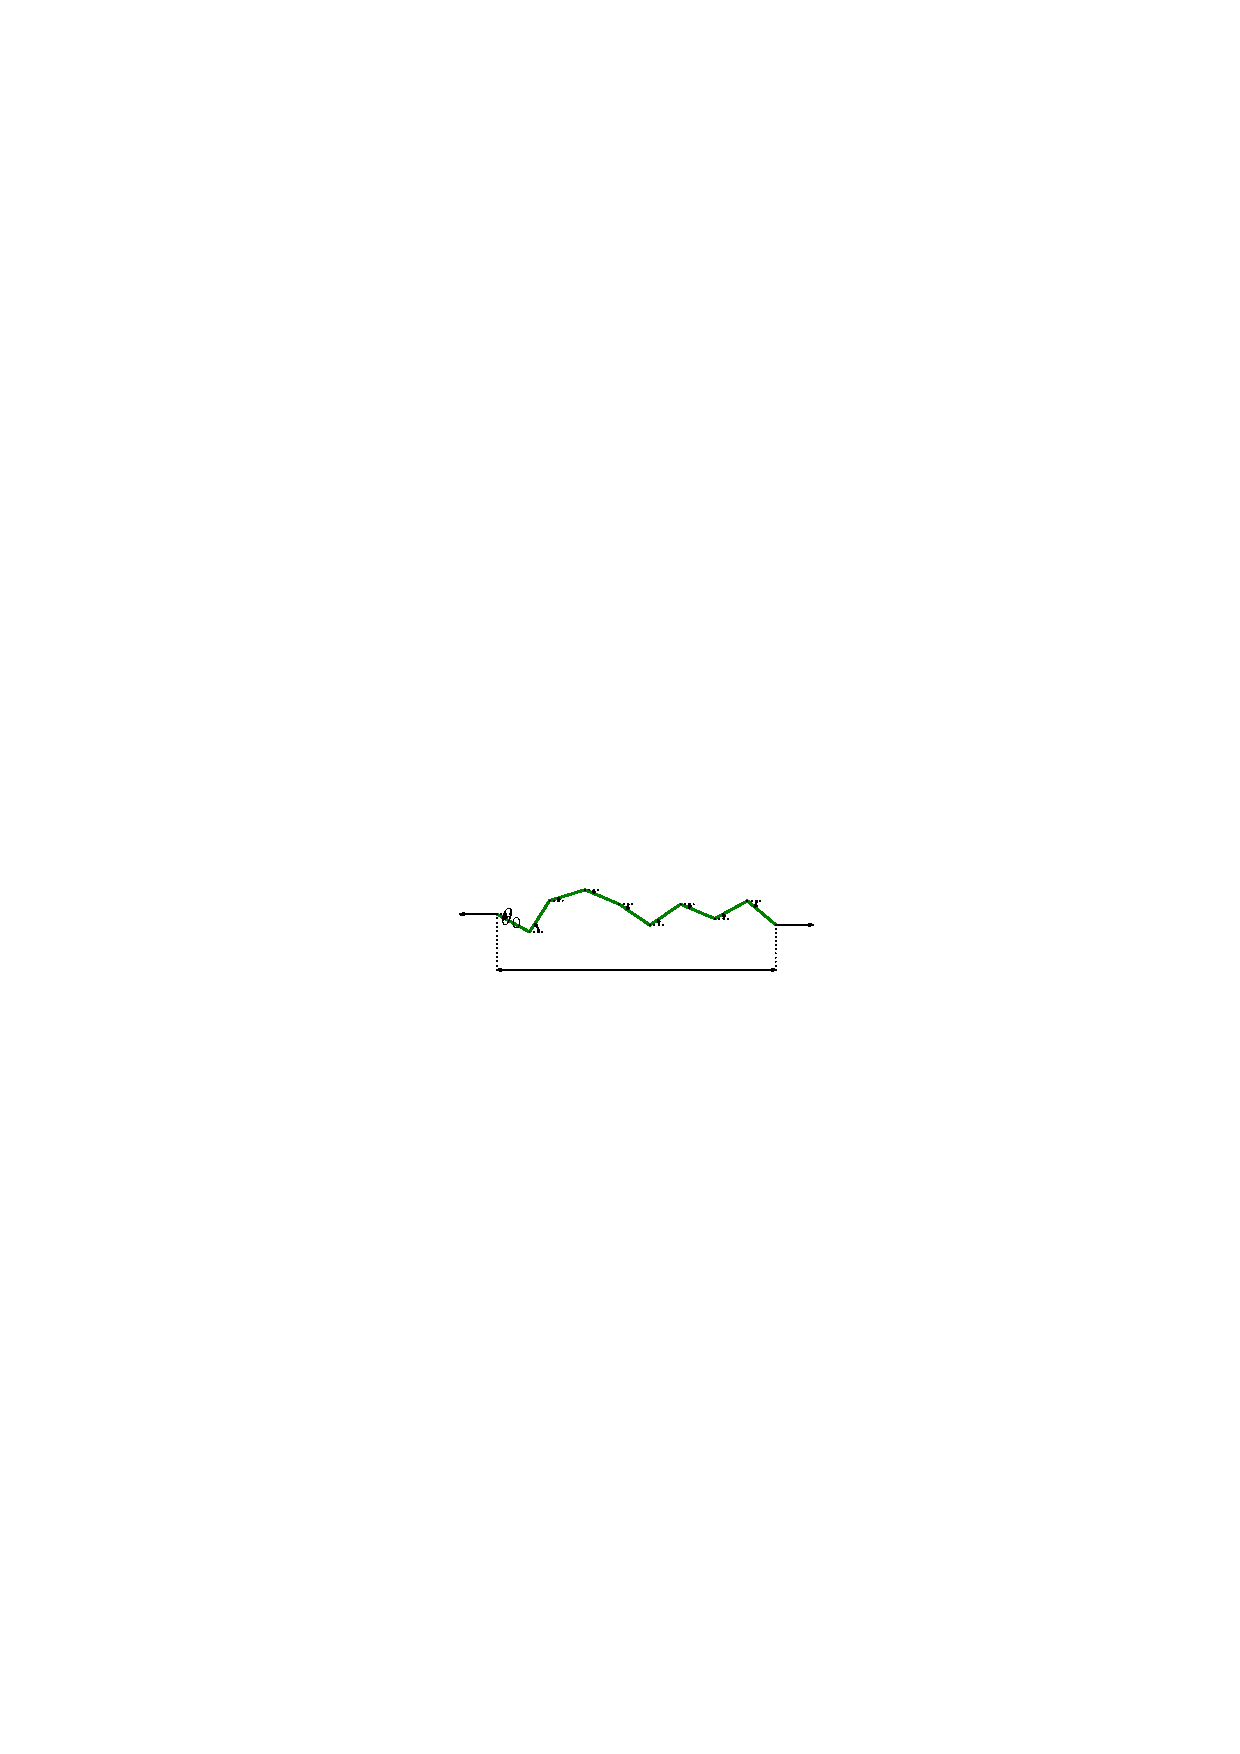
\includegraphics[width = 12cm]{./Eadn_1_fig.pdf}
 % Eadn_1_fig.pdf: 0x0 pixel, 300dpi, 0.00x0.00 cm, bb=
 \caption{Modèle de chaîne librement jointe}
 \label{fig: adn_1}
\end{figure}
\noindent
Une molécule d'ADN (supposée plane) peut être modélisée\footnote{D'après centrale-supelec IPT commune 2019 \og\'Elasticité d'un brin d'ADN\fg (partie IV).} par une \og chaîne librement jointe\fg dans laquelle des segments rigides (appelés \emph{monomères}) sont liés à leurs extrémités et librement orientables aux points de jointure. On appelle \emph{conformation} de la molécule sa configuration géométrique. En l'absence d'action extérieure, l'orientation de chaque segment (défini par $\theta_i$) par rapport à ses voisins est aléatoire et toutes les conformations sont équiprobables.\newline
Ce texte propose une simulation de ce modèle selon la méthode dite de \og Monte-Carlo\fg. Pour une conformation et une force données, une énergie est calculée. Puis des changements aléatoires de conformation sont effectués. Ils convergent vers un état naturel de la molécule.\newline
Pour un brin d'ADN soumis à une force $\overrightarrow{F}$ imposée, l'énergie mécanique $E$ développée pour étendre la molécule s'écrit
\[
 E = - z F
\]
où $F$ est l'intensité de la force et $z$ l'allongement de la molécule dans la direction de la force (fig \ref{fig: adn_1}).\newline
La simulation démarre à partir d'une conformation aléatoire du brin d'ADN.
\begin{enumerate}
 \item \'Ecrire une fonction d'entête
\begin{verbatim}
    def conformation(n: int):
\end{verbatim}
qui renvoie une liste de longueur $n$ correspondant à l'orientation (angles $\theta_i$) de chaque segment. Cette liste représente une conformation de la molécule.
  \item \'Ecrire une fonction d'entête
\begin{verbatim}
 def allongement(theta, l: float):
\end{verbatim}
qui renvoie l'allongement $z$ de la chaîne dans la conformation $\theta$ pour une longueur de segment $l$.
\end{enumerate}

La modification de la conformation se fait en modifiant de façon aléatoire $k$ angles successifs, $k$ étant un paramètre ajustable.
\begin{enumerate}[resume]
 \item \'Ecrire une fonction d'entête
\begin{verbatim}
 def nouvelle_conformation(theta, k: int):
\end{verbatim}
qui renvoie une nouvelle conformation en modifiant $k$ valeurs consécutives à partir d'un indice aléatoire.
\end{enumerate}
L'agitation thermique de la molécule tend à la désordonner aléatoirement alors que la force extérieure tend à aligner les brins (diminution de l'énergie). Les deux phénomènes se stabilisent vers une situation où force et allongement sont liés. L'algorithme vise à déterminer cet équilibre statistique.\newline
\`A partir d'une conformation d'énergie calculée $E_1$ (conformation courante), une nouvelle conformation est crée et son énergie $E_2$ est calculée. Cette nouvelle conformation peut être conservée (et devenir la conformation courante) ou abandonnée:
\begin{itemize}
 \item si $E_2 < E_1$, la nouvelle conformation est conservée et devient la conformation courante;
 \item si $E_1 \leq E_2$, la nouvelle conformation est conservée avec la probabilité 
\[
 P = \exp \left( \frac{E_1 - E_2}{k_B\,T}\right) .
\]
 Elle devient alors la conformation courante.
\end{itemize}
\begin{enumerate}[resume]
 \item \'Ecrire une fonction d'entête
\begin{verbatim}
 def selection_conformation
     (thetaA, thetaB, F: float, l: float, T: float):
\end{verbatim}
qui prend en paramètres deux conformations (\texttt{thetaA} désignant une conformation initiale et \texttt{thetaB} une nouvelle conformation) et qui renvoie la conformation conservée. Les autres paramètres sont l'intensite de la force \texttt{F}, la longueur d'un segment \texttt{l} et la température \texttt{T}.
\end{enumerate}
Rappelons la définition de la variance d'une famille de $p$ nombres $(x_1, \cdots, x_p)$.
\[
 \overline{x} = \frac{1}{p}\sum_{i=1}^{p}x_i, \hspace{0.5cm} V = \frac{1}{p}\sum_{i=1}^{p}(x_i - \overline{x})^2 = \frac{1}{p}\sum_{i=1}^{p}x_i^2 - \overline{x}^2.
\] 
\begin{enumerate}[resume]
 \item  On considère une famille de $p+1$ flottants $x_1, \cdots, x_{p+1}$ pour laquelle on connait la moyenne $x$ et la variance $V$ de la famille  $(x_1, \cdots, x_p)$ des $p$ premiers termes. On veut calculer la variance de la famille $(x_2,\cdots, x_{p+1})$ des $p$ termes suivants.
Comment le faire avec un nombre d'opérations (additions et multiplications) indépendant de $p$ ?
\end{enumerate}
La méthode de Monte-Carlo consiste à former des centaines de conformations successives conservées sous les conditions précisées plus haut. On considère que l'algorithme a convergé lorsque la variance de l'allongement du brin sur les 500 dernières conformations est inférieure à un paramètre $\varepsilon$ de la simulation.
\begin{enumerate}[resume]
 \item \'Ecrire une fonction d'entête
\begin{verbatim}
 def monte_carlo(F, n, l, T, k, eps):
\end{verbatim}
qui simule l'application d'une force de traction d'intensité \texttt{F} sur un brin d'ADN de \texttt{n} monomères de longueur \texttt{l} à la température \texttt{T}. Les arguments \texttt{k} et \texttt{eps} sont des paramètres de la simulation telle que définie plus haut.\newline
La fonction renvoie l'allongement moyen des 500 dernières conformations une fois la convergence atteinte.
\end{enumerate}
\emph{Indication.} Compte tenu du nombre d'itérations envisagées, on n'enregistrera pas toutes les étapes intermédiaires. On utilisera une \emph{file} pour stocker les données. Une file est une structure de données où les premiers éléments entrés sont les premiers qui en sortent (\og First In First Out \fg).\newline
On émulera une file à l'aide d'une liste en utilisant les méthodes \texttt{append} pour entrer et \texttt{pop(0)} pour sortir.\newline
On rappelle que \texttt{L.append(x)} ajoute \texttt{x} à la fin de \texttt{L} et ne renvoie rien et que \texttt{L.pop(0)} renvoie le premier terme de \texttt{L} et le supprime de la liste.\newline
Dans la bibliothèque \texttt{random}: la fonction \texttt{randrange(a,b)} renvoie un entier aléatoire entre \texttt{a} et \texttt{b - 1} où \texttt{a} et \texttt{b} désignent des entiers; la fonction \texttt{random()} renvoie un flottant entre 0 et 1 (distribution uniforme).

